\documentclass{article}
\usepackage{inputenc}
% 中文排版
\usepackage{ctex}
\usepackage[dvipsnames, svgnames, x11names]{xcolor}
% 超链接
\usepackage[colorlinks]{hyperref}
% 书签
\usepackage{bookmark}
% 设置页边锯
\usepackage{geometry}
\geometry{left=2cm,right=2cm,top=2.5cm,bottom=2.5cm}
% 高亮
\usepackage{soul}
% 代码块
\usepackage{listings}
% 用来设置附录中代码的样式
\lstset{
    basicstyle = \zihao{-5}\ttfamily,
    keywordstyle = \zihao{-5}\ttfamily\color{blue},
    commentstyle = \ttfamily\color{Green},
    stringstyle = \ttfamily\color{BrickRed},  % 字符串风格
    flexiblecolumns,
    numbers = left,   % 行号的位置在左边
    showspaces = false,  % 是否显示空格,显示了有点乱,所以不现实了
    numberstyle = \zihao{-5}\ttfamily\color{TealBlue},
    showstringspaces = false,
    captionpos = t,
    frame = shadowbox
}
% 图片
\usepackage{graphicx}
\usepackage{caption}
\usepackage{subfigure}
\usepackage{float}

% 跨页表格
\usepackage{longtable}

\title{Latex入门}
\author{陈昊天}
\date{2019年4月26日}

\begin{document}
    \maketitle
    \tableofcontents
    \section{环境配置}
        \subsection{texlive的安装}
            \textbf{texlive}是进行Tex排版最关键的软件之一,其作用相当于sdk,是编译和运行Latex必须的。你可以转到\textbf{texlive}官网(\url{http://tug.org/texlive/})进行下载,但这种方式并不是很推荐。推荐使用国内的镜像源下载其开源的iso镜像。例如清华开源镜像站(\url{https://mirrors.tuna.tsinghua.edu.cn/CTAN/systems/texlive/Images/})下载\textbf{}{texlive.iso}文件。
            下载完成texlive.iso文件后,使用虚拟光驱软件(或者系统自带的打开),用管理员运行里面的文件\hl{install-tl-advanced.bat},之后可以打开\hl{N. of collections}选项,去掉不经常使用的语言包(建议保留中文和英文)和texworks编辑器,具体操作方法请参考教程。\footnote{参考自知乎教程\heiti{最新TeXLive 环境的安装与配置}(\url{https://zhuanlan.zhihu.com/p/64555335})}
        \subsection{vscode环境配置}
            网上有很多Latex编辑器可以选择,但是本文主要讲解在vscode上进行环境配置的方法。打开vscode,在扩展商店中搜索\hl{Latex Workshop},进行安装,基本上只要这么一个扩展就足够使用了。接下来最关键的一步是修改vscode的环境配置。首先按下快捷键Ctrl + Shift + P,选择\hl{Open Settings(Json)}选项,用附带的文件settings.json覆盖原来的配置。覆盖方式为将第一个括号内的内容复制到设置的第一个括号内结尾处,然后删掉之前重复的设置项,然后保存\footnote{参考自知乎问题回答\heiti{有哪些好的 LaTeX 编辑器?}(\url{https://www.zhihu.com/question/19954023/answer/676316395})}。
        \subsection{开始第一个Latex项目}
            由于.tex文件编译和运行时需要生成一系列文件,建议专门创建一个文件夹进行文档编写。首先创建一个文件夹Hello,然后新建一个文件hello.tex,在文件内输入下列文本。
            % 代码块
            \lstinputlisting[language=tex]{texs/hello1.tex}
            \textit{代码文件见\url{./texs/hello1.tex}}

            之后选择选项卡Latex->commands->Build Latex project->Recipe:xelatex,进行编译。然后点击上方View Latex PDF File,稍等便可将会在右侧显示编译好的Latex文件。

            \begin{figure}[H]
                \centering
                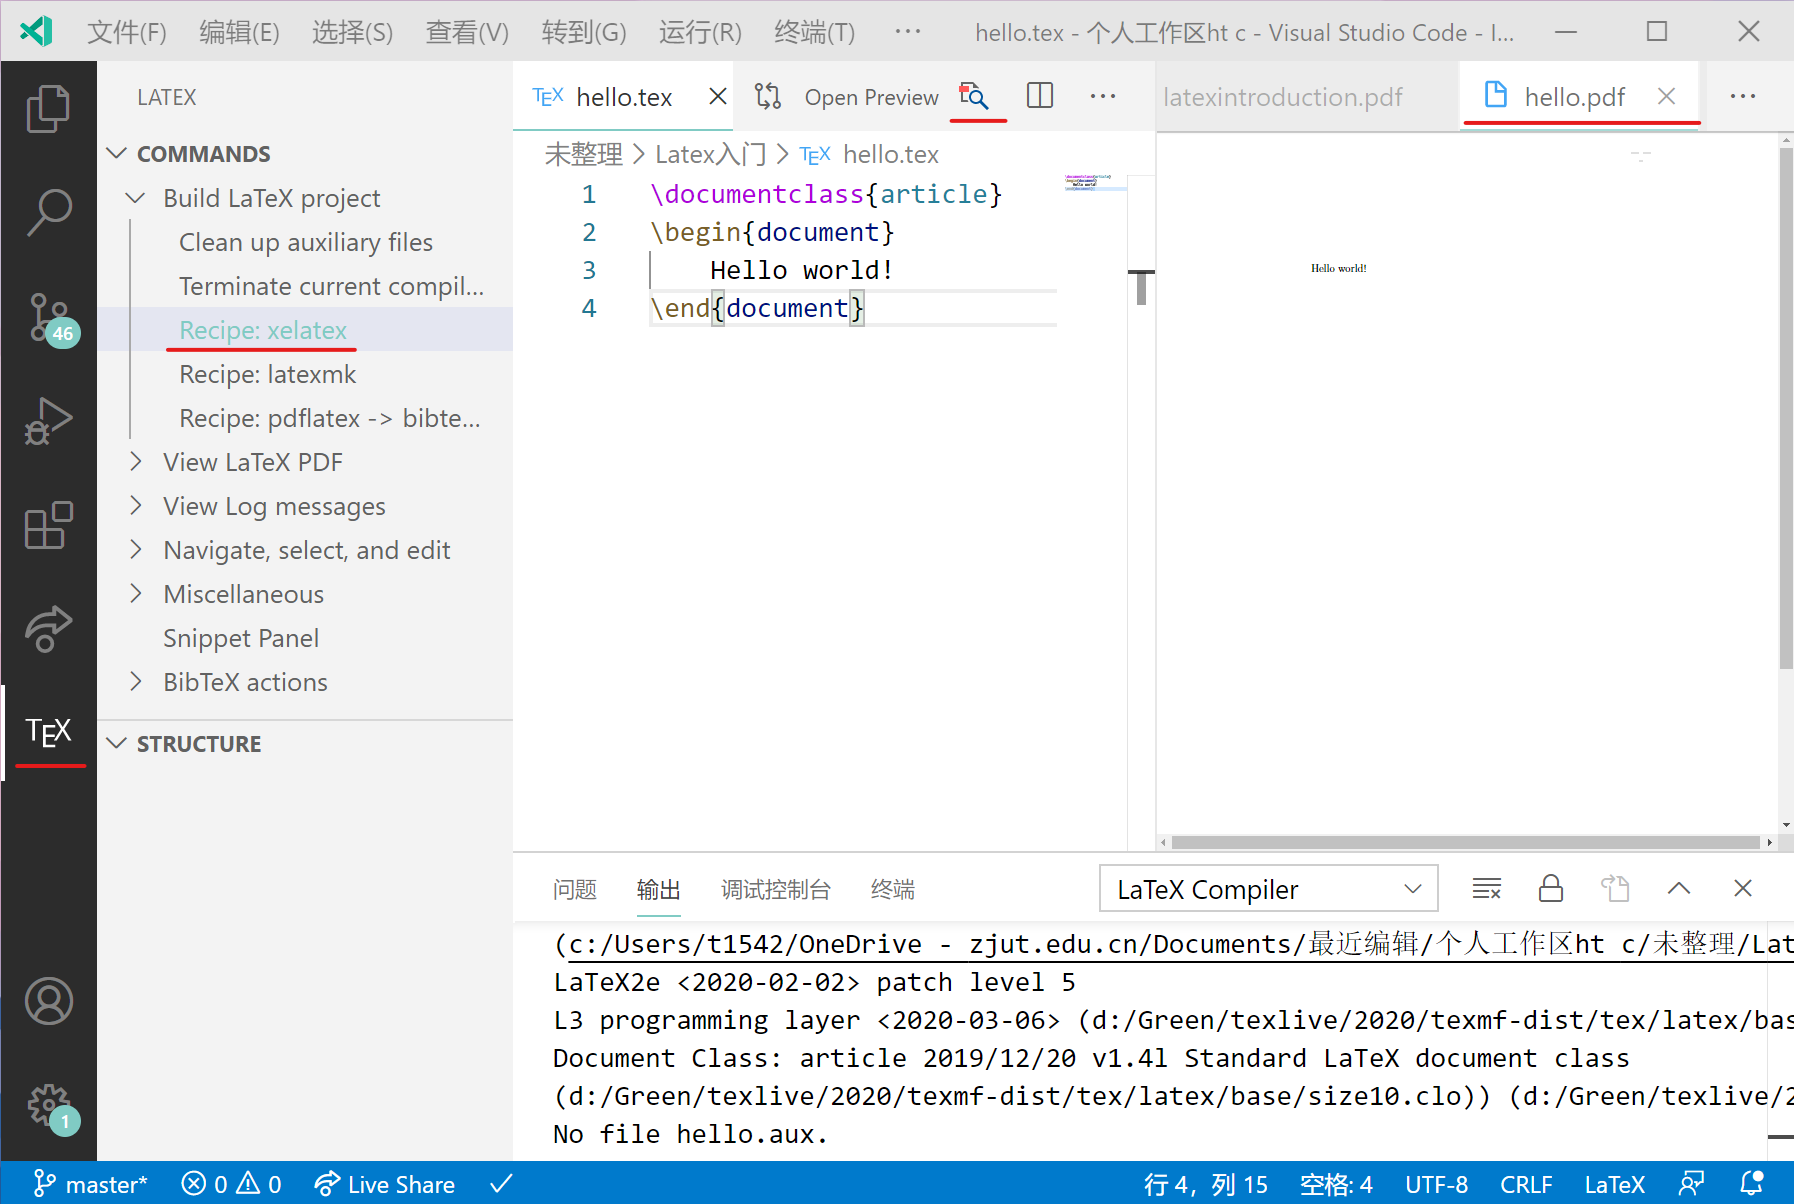
\includegraphics[width=0.8\textwidth]{snaps/snap1.png}
                \caption{编写Hello.tex文件并编译}
                \label{snap1}
            \end{figure}

            学习一门新的技能,最麻烦的地方在开头的环境配置,只要你能够在vscode正确编译并运行,那么你之后遇到的麻烦将会少很多,因为有啥问题查看错误报告。下面将会在此基础上讲解Latex的各种特性。
    \section{Latex宏}
        \subsection{Latex宏命令}
        Latex到处充满了宏命令,宏也是Latex中最核心的内容,一般宏分为命令宏,单行宏,段落宏\footnote{这里的宏分类并不是严谨的,这里按照宏实现的功能进行分类,是为了便于理解。},命令分别如下。

        \lstinputlisting[language=tex]{texs/tutoral1.tex}
        \textit{代码文件见\url{./texs/tutoral1.tex}}

        熟练的使用宏命令可以让Latex文档的编写更加轻松,其中最基本的宏命令是关于排版的命令,将会在排版章节讲解。

        \subsection{Latex环境}
        有时候我们会提到环境这个词,这个其实我们在写文章的时候就会不自觉的用到。有时候,基于内容的不同便会使用不同的环境。

        \lstinputlisting[language=tex]{texs/hello1.tex}
        \textit{代码文件见\url{./texs/hello1.tex}}

        例如上面最简单的一个文档(应该没有比这更简单的了)第2-4行之间的内容就属于document环境。这个时候代码的执行和渲染按照document来执行。之后使用到的插入表格和图片均会使用到相应的Latex环境。

        \subsection{Latex宏包}
        原生的Latex支持的内容并不是很多,最简单的一点,就是Latex不支持中文,因此,要编写排版优雅,具有一定美观性的文档肯定离不开\textbf{宏包},有些包是官方给出,也有些是第三方开发的,这些宏包组合起来,可以实现各种各样的功能。

        \subsubsection{导入宏}
            有时候你在写一句宏指令时会发现没有自动提示或者编译时出错,往往是没有导入正确的宏的结果,导入宏用到命令是$\backslash$usepackage$\lbrace$packagename$\rbrace$,此命令理论上可以放置在任意的位置,但推荐放在document区域之前,例如下文的代码。如果把中文排版的删掉,编译后并不会出错,但其中的中文字符将不会显示。

            \lstinputlisting[language=tex]{texs/hello2.tex}
            \textit{代码文件见\url{./texs/hello2.tex}}

        \subsubsection{常用的宏包}
            其中,在中文编辑中,ctex宏包是最重要的一个宏包\footnote{ctex不仅仅使latex支持中文,而且加了很多的功能,让Latex排版符合中国人的习惯。},而且其已经形成了一个完整的生态。可以在CTAN相关的网站进行查看。例如CTEX在线文档(\url{http://www.ctex.org/documents/packages/})。

            下面将列出经常使用到的宏包,某些常用功能的使用将会在后续的教程中编写。

            % \begin{table}[H]
            %     \centering
            %     \begin{tabular}{p{2cm}p{3.5cm}p{9cm}}
            %         \hline
            %         宏包 & 功能 & 功能说明 \\
            %         \hline
            %         ctex & tex的中文发行版 & 如果文档是中文的,则必须使用此宏包。 \\
            %         inputenc & 输入的编码 & 用于控制输入的编码,在ctex中一般不会使用,用于解决西文特殊符号导致编码错误的问题。\\
            %         geometry & 页面布局 & 用于设置页边距,页眉和页脚的位置等。(一般默认的页边距太大了。) \\
            %         multicol & 分栏 & 用于对文章的特殊区域进行分栏的操作。 \\
            %         float & 设置浮动元素 & 可以自定义浮动样式,使部分元素脱离正确的文档流位置。 \\
            %         caption & 标签 & 用于设置表格、图片和其他内容的标签 \\
            %         graphicx & 插入图像扩展版本 & 用于插入图像 \\
            %         subfigure & 插入子图 & 用于在一个区域内插入多张图片,常常和graphicx一起使用。 \\
            %         amsmath amssymb & 数学公式 & 扩用于扩展Latex的公式系统,以提供更多中公式的显示。 \\
            %         natbib & 参考文献 & 扩展Latex的参考文献功能。 \\
            %         hyperref & 超链接 & 在文档中插入超链接 \\
            %         soul & 文本修饰 & 提供了多种文本修饰的效果 \\
            %         listings & 代码块 & 支持在Latex中插入代码和高亮代码 \\
            %         \hline
            %     \end{tabular}
            %     \caption{常用的宏包}
            % \end{table}

            \begin{center}
                \begin{longtable}{p{2cm}p{3.5cm}p{9cm}}
                        \hline
                        宏包 & 功能 & 功能说明 \\
                        \hline
                    \endfirsthead
                        \hline
                        宏包 & 功能 & 功能说明 \\
                        \hline
                    \endhead
                        \hline
                    \endfoot
                        \hline
                        \caption{常用的宏包}
                    \endlastfoot
                    ctex & tex的中文发行版 & 如果文档是中文的,则必须使用此宏包。 \\
                    inputenc & 输入的编码 & 用于控制输入的编码,在ctex中一般不会使用,用于解决西文特殊符号导致编码错误的问题。\\
                    geometry & 页面布局 & 用于设置页边距,页眉和页脚的位置等。(一般默认的页边距太大了。) \\
                    multicol & 分栏 & 用于对文章的特殊区域进行分栏的操作。 \\
                    float & 设置浮动元素 & 可以自定义浮动样式,使部分元素脱离正确的文档流位置。 \\
                    caption & 标签 & 用于设置表格、图片和其他内容的标签 \\
                    graphicx & 插入图像扩展版本 & 用于插入图像 \\
                    subfigure & 插入子图 & 用于在一个区域内插入多张图片,常常和graphicx一起使用。 \\
                    amsmath amssymb & 数学公式 & 扩用于扩展Latex的公式系统,以提供更多中公式的显示。 \\
                    natbib & 参考文献 & 扩展Latex的参考文献功能。 \\
                    hyperref & 超链接,内部连接 & 在文档中插入超链接 \\
                    bookmark & pdf书签系统 & 用于在pdf中加入书签系统,以便于浏览与翻阅,包含了hyperref的功能。请在hyperref后声明。\\
                    soul & 文本修饰 & 提供了多种文本修饰的效果 \\
                    listings & 代码块 & 支持在Latex中插入代码和高亮代码 \\
                    longtable & 长表格 & 用于在Latex中制作跨页的表格(一般Latex的表格不支持跨页) \\
                \end{longtable}
            \end{center}

    \section{Latex基本语法}
        \subsection{内容与排版}
            \subsubsection{主标题}
                Latex默认提供了快速编写标题的命令,标题样式是默认的,如果需要自定义标题,需要使用其他的宏包,但是一般默认的已经够了。

                \lstinputlisting[language=tex]{texs/hello3.tex}
                \textit{代码文件见\url{./texs/hello3.tex}}

            \subsubsection{标题与内容}
                Latex默认支持多级标题与内容,其中$\backslash$section$\lbrace$section-title$\rbrace$将会插入一级标题。$\backslash$subsection$\lbrace$subsection-title$\rbrace$将会插入二级标题。$\backslash$subsubsection$\lbrace$subsubsection-title$\rbrace$将会插入三级标题。例如下列代码。

                \lstinputlisting[language=tex]{texs/hello4.tex}
                \textit{代码文件见\url{./texs/hello4.tex}}

                \begin{figure}[H]
                    \centering
                    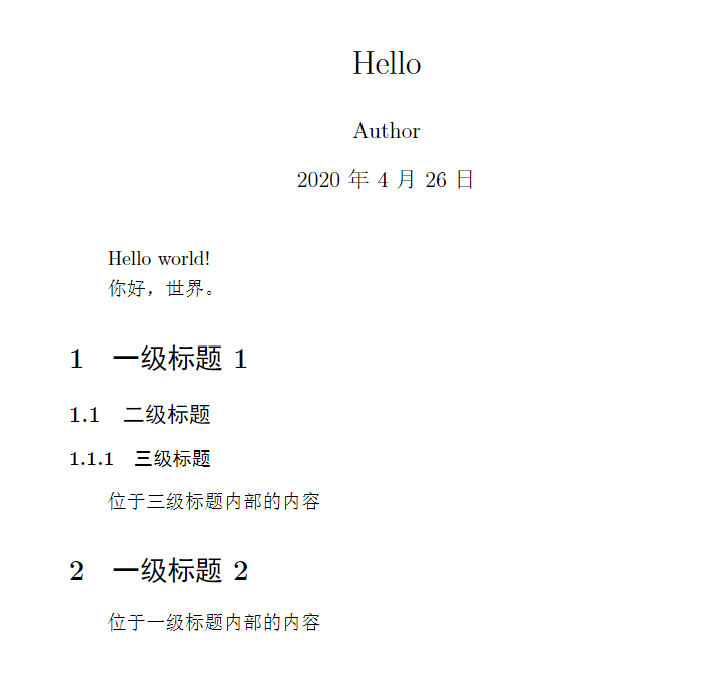
\includegraphics[width=0.6\textwidth]{snaps/snap2.png}
                    \caption{标题与内容效果图}
                    \label{snap2}
                \end{figure}

                其他关于段落有一篇知乎文章\textbf{LaTeX入门(五)——段落}(\url{https://zhuanlan.zhihu.com/p/56127244})写得很好。

            \subsubsection{目录}
                Latex支持自动导出目录,只需要加入$\backslash$tableofcontents语句然后编译即可\footnote{由于Latex的相关原因,编译一次可能并没有效果,需要编译两次及以上,这个问题将在后面讨论}。

                \lstinputlisting[language=tex]{texs/hello5.tex}

                \begin{figure}[H]
                    \centering
                    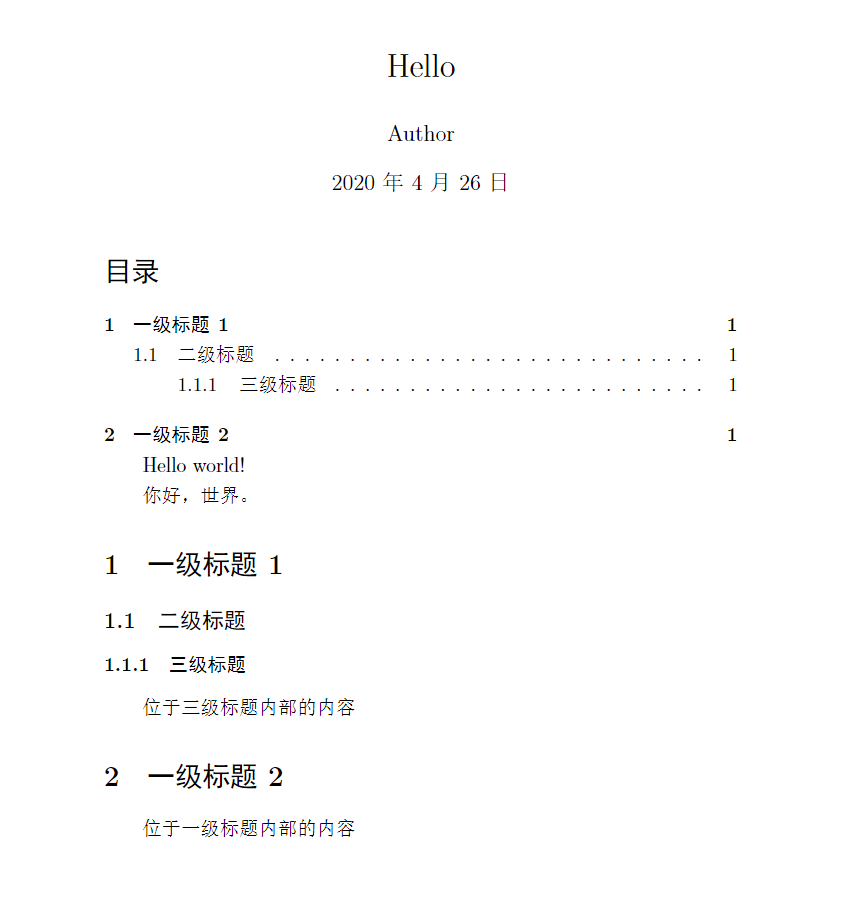
\includegraphics[width=0.6\textwidth]{snaps/snap3.png}
                    \caption{目录效果图}
                    \label{snap3}
                \end{figure}

                当然,此时点击目录并没有什么效果,如果要在目录上生成跳转链接,只需要导入hyperref宏包即可,具体步骤请看\hyperlink{author}{在文档内部创建锚点与跳转}。

                当然,当你改变文档的目录结构(例如添加一个section,删除一个section)时,第一次编译时目录并不会跟着刷新,关于此问题请转至常见问题\hyperlink{norefresh-toc}{更新后目录没有刷新}部分。

            \subsubsection{文档类型和样式}
                Latex为不同的文档类型预置了不同的基础样式,因为文章的内容,排版方式有所不同。有时候我们需要的是一篇短小的文章,有时候我们会用Latex编写(当然一般不会这么做。)

                Latex排版系统虽然非常优秀,让编写者可以关注于内容,而不需要费心思关心与排版,然而这是基于Latex内置或者在其他样式的基础之上的。因此,要定制Latex还是比较麻烦的,这部分属于Latex高级语法,一般对于日常使用而言,可以直接套用网上流传的模板,可以减轻很多的工作。

                当然,在编写文档时,我们可能还会遇到另外几个问题。这些问题将会在\hyperlink{other-question}{常见问题}有所说明。

                一般来说,文档类型很多,而且用户可以自定义文档类型。比如一般我们再写论文时第一句就会写上$\backslash$documentclass$\lbrace$article$\rbrace$,这个便是声明该文章的样式了。一般来说,常见的有article,report,book三种,分别对应短篇幅,中篇幅,长篇幅。
            \subsubsection{include命令}
                include命令,顾名思义,和html文档一样,在一个Latex文档内,可以使用include命令导入另一个Latex文档,这就相当于文档替换的作用。体现了部分的模块设计思想。只要使用$\backslash$include$\lbrace$url$\rbrace$即可使用此功能。
                
                例如,当你需要写一篇很长的书籍时(只有这个合适的例子了),总不可能在一个.tex文件内写所有的内容,这时候,一般main.tex文件就作为主.tex文件,起着排版和设计样式的作用。
            \subsubsection{页面布局}
                这部分在知乎专栏文章\textbf{LaTeX入门(七)——页面设置}(\url{https://zhuanlan.zhihu.com/p/56405574})有详细介绍。
            \subsubsection{小技巧:快速定位元素}
                Latex预览状态下的pdf不想markdown文档一样,会和源代码同步对齐内容。两者滚动条是分离的。这里有个小技巧。当使用ctrl+鼠标左键点击pdf中的文字时,会直接跳转到源码中的相应内容。这对于篇幅过长的文档的元素定义有奇效。
        \subsection{文字效果}
            这部分内容需要进一步地更新
            \subsubsection{常见修饰效果}
                常见的修改字体修饰效果,例如斜体、粗体、设置字体族可以直接查看知乎文章教程\textbf{LaTeX入门(四)——文字}(\url{https://zhuanlan.zhihu.com/p/56069161})
                其中常用的命令有设置粗体$\backslash$textbf$\lbrace$content$\rbrace$,设置斜体$\backslash$textit$\lbrace$content$\rbrace$等。



            \subsubsection{着重号}
            \subsubsection{首字下沉}
            \subsubsection{强调色}
        \subsection{表格与图片}
            这部分内容需要进一步地更新
            \subsubsection{传统表格}
            \subsubsection{长表格,多页表格}
            \subsubsection{图片}
        \subsection{书签、引用、链接}
            \subsubsection{创建书签}
                \footnote{参考自csdn教程Latex下关于bookmark包乱码修正的注记\url{https://blog.csdn.net/newdriver2783/article/details/79658056}}
                当我们导出pdf文件再在浏览器上打开后,我们会发现并没有生成目前,这是怎么回事呢。要解决这个问题,我们只要导入bookmark包就可以了。此时,你会发现打开pdf后有书签了,而且点击目录的相应位置会跳转到文档的相应的位置。当然,有时候我们希望这种链接显眼一些。相关内容请看\hyperlink{changelinkcolor}{改变链接的颜色}。

                \lstinputlisting[language=tex]{texs/hello6.tex}
                \textit{代码文件见\url{./texs/hello6.tex}}

            \hypertarget{author}{}
            \subsubsection{链接系统}
                必须导入宏包$\backslash$hyperref。
                
                \lstinputlisting[language=tex]{texs/link1.tex}
                \textit{代码文件见\url{./texs/link1.tex}}

            \hypertarget{changelinkcolor}{}
            \subsubsection{改变链接的颜色}
                需要改变的链接,必须要导入宏包$\backslash$hyperref。然后可以使用$\backslash$hypersetup进行颜色的定制。

                \lstinputlisting[language=tex]{texs/linkcolor.tex}
                \textit{代码文件见\url{./texs/linkcolor.tex}}

                \begin{figure}[H]
                    \centering
                    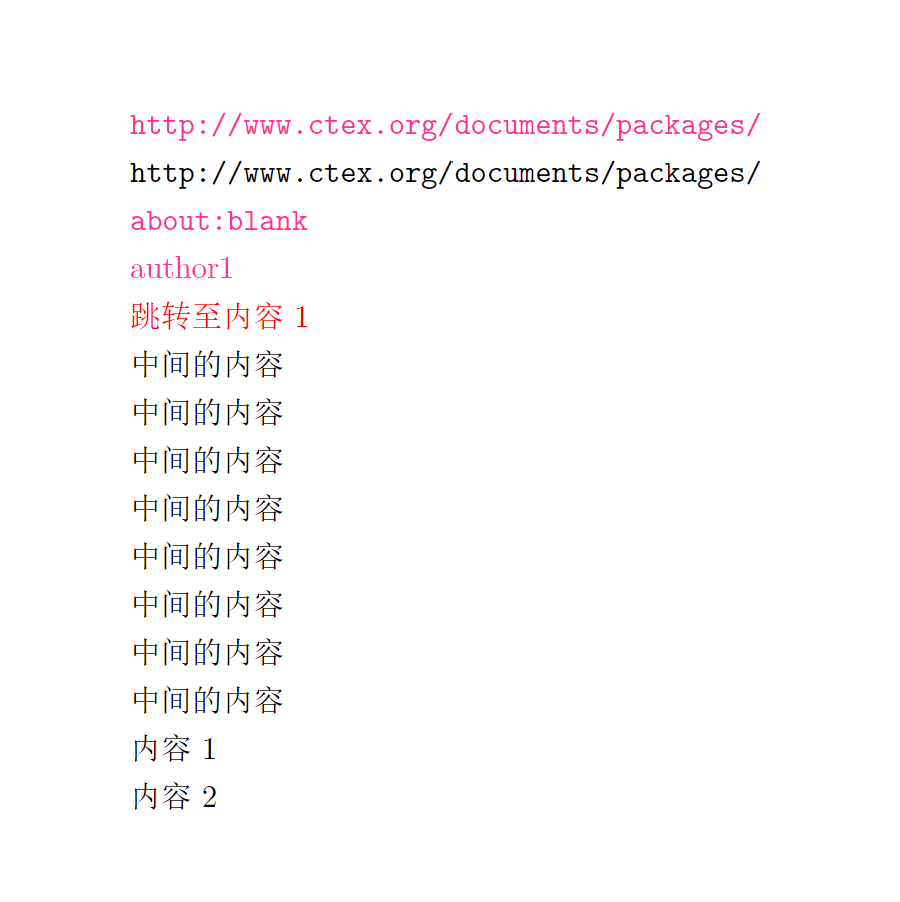
\includegraphics[width=0.6\textwidth]{snaps/snap4.png}
                    \caption{链接效果图}
                    \label{snap4}
                \end{figure}

        \subsection{页面其他元素}
            这部分代码需要进一步更新
            \subsubsection{标签caption}
            \subsubsection{注释}
            \subsubsection{参考文献}
        \hypertarget{other-question}{}
        \subsection{常见问题}
            \hypertarget{norefresh-toc}{}
            \subsubsection{更新后目录没有更新}
                目录(其实就是文章的结构)其实是记录在当前路径与本文件同名的.toc文件中的,打开就会看到很多看起来向概要的latex代码。这便是文章的结构。改变文章的目录结构后第一次编译时,会发生.toc更新后无法及时呈现在latex文档上的问题,这时候多编译几次这个问题就可以得到有效解决。
            \subsubsection{文档没有显示问题但无法通过编译}
                关于这一点,我无法给出究竟是什么原因。但在我自己的电脑上,也出现过几次问题。

                第一种是使用了某些软件打开了pdf文件,导致文件被锁定,无法通过编译。第二种是电脑的内存占用过高,而显示Memory Exhasted的警告(看来这个软件确实内存占用挺高的,特别是编译的时候。)
    \section{代码块}
        待完善的内容
    \section{Latex公式系统}
        待完善的内容
    \section{扩展}
        \subsection{颜色}
    \section{自定义样式}
        太难了,暂时没有打算写。
    \section{代码系统}
        其实也没有必要写。
    \section{测试效果}
        \subsection{代码高亮}
            下面将测试python代码的高亮情况。

            \lstinputlisting[language=python]{others/fibonacci.py}


\end{document}
